\section{Basics of Copula Theory}

\begin{lem}[Frechet bounds]
	
	Copula has the following bounds:
	\begin{equation} \label{eq:frechet_bound}
		\max \left(0, \sum_{i=1}^{d} u_i + 1 -d \right) \le C(u_1,...,u_d) \le \min(u_1,...,u_d).
	\end{equation}
\begin{proof}
	Note that $C(u1,...,u_d) = \bP( \bigcap_{i=1}^{d} \{U_i \le u_i\})$ and 
	\[\bigcap_{i=1}^{d} \{U_i \le u_i \subset \{U_i \le u_i \}, \text{ for } i=1,...,d.\]
	The second inequality (upper bound) follows then by combining these two facts.
	For the lower bound, re-write the joint CDF as follows:
	\[ C(u_1,..., u_d) = 1- \bP\left( \bigcup_{i=1}^{d} \{U_i > u_i\}\right).\]
	One has
	\[\bP\left( \bigcup_{i=1}^{d} \{U_i > u_i\}\right) \le \sum_{i=1}^{d} \bP( U_i > u_i) = d - \sum_{i=1}^{d} u_i.\]
	Combining ... and the fact that $C(u)\ge 0$, yields:
		$\max(0, \sum_{i=1}^{d} u_i + 1 -d) \le C(u_1,...,u_d)$.
\end{proof}
\end{lem}

\begin{thm}[{\bf Invariance via strict monotonic transformation}]
	Let $X=(X_1,...,X_d)$ be a multivariate random variable with copula $C$ and $T_i,\ i=1,...d$ be strictly increasing functions. Then 
	\[Y = (Y_1, ..., Y_d) := (T_1(X_1), ..., T_d(X_d))\]
	has the same Copula as X, i.e. {\bf Copula is invariant under strict monotonic transformation}.
	
\end{thm}
\begin{proof}
	Denote by $G, G_1,..., G_d$ and $F, F_1, ...,F_d$ joint- and marginal CDFs of$X$ and $Y$, respectively. We need to prove that
	\begin{equation} \label{eq:monotrans}
		G(y_1, ..., y_d) = C(G_1(y_1),...,G_d(y_d)).
	\end{equation}
It follows from the definition of $Y_i, \ i=1,...,d$ that 
	\begin{equation} \label{eq:monotrans0}
			G_i(y_i) =  \bP(T_i(X_i) \le y_i ) = \bP(X_i \le T_i^{-1}(y_i)) = F_i(T_i^{-1}(y_i)).
	\end{equation}
 Let's work out the joint CDF of $Y$:
 \begin{align}
 	\label{eq:monotrans1}
 \nonumber	G(y_1, ..., y_d)& = \bP(Y_1 \le y_1, ..., Y_d \le y_d) \\ \nonumber
 	&= \bP(T_1(X_1)\le y_1,..., T_d(X_d)\le y_d) \\ \nonumber
 	&= \bP(X_1 \le T_1^{-1}(y_1),...,X_d \le T_d^{-1}(y_d))\\ \nonumber
 	&= F(T_1^{-1}(y_1),..., T_d^{-1}(y_d))\\
 	& = C(F_1(T_1^{-1}(y_1)),...,F_d(T_d^{-1}(y_d))).
 \end{align}
Combining \eqref{eq:monotrans0} and \eqref{eq:monotrans1} yields \eqref{eq:monotrans}. Note that the last equality in \eqref{eq:monotrans1} is due to the property of Copula.
\end{proof}
\textcolor{red}{\bf TODO: provide a generic description or pseudocode how to construct a multivariate rv with a certain dependence structure and given marginal cdfs from scratch.}

\begin{algorithm}
	\SetAlgoLined
	\KwIn{Marginal CDFs, $F_1,..., F_d$ and a dependence structure, e.g. via an explicit Copula.}
	\KwOut{A multivariate rv $X$ with marginal CDFs given by $F_i, \ i=1,..., d$ and the given dependence structure.}	
	\caption{Construction of a multivariate rv with given marginal CDFs and dependence structure.}
	{\bf Step 1:} Construct $U=(U_1,...,U_d)$ where $U_i\sim \cU(0,1), \ i=1,..., d$ that has joint CDF $C(u)$.\\
	{\bf Step 2:} Work out the inverse functions of the marginal CDFs: $F_1,..., F_d$. Sometimes a numerical approximation is required when an analytical form is not available or tractable to work with.\\
	{\bf Step 3:} Obtain $X=(X_1,..., X_d)$ where 
	\begin{equation}
		X_i = F_i^{-1}(U_i), \ i=1,...,d.
	\end{equation}
	The rv $X$ has the given marginal cdfs $F_i,\ i=1,...,d$ and Copula $C$.
	\label{algo:genericsim}
\end{algorithm}

\begin{rem}
	Some preliminary results are necessary here to ease understanding, e.g. $F_X^{-1}(U) \sim \F_X$, $F_X(X) \sim \cU(0,1)$. 
	
	Step 1 in Algorithm~\ref{algo:genericsim} involves simulating the multivariate uniform rv $U$ with a given joint CDF. \remend 
\end{rem}

Let $X$ be a random variable with cumulative distribution function (cdf) $F_X$. Then
\begin{wrapfigure}{r}{3.5cm}
		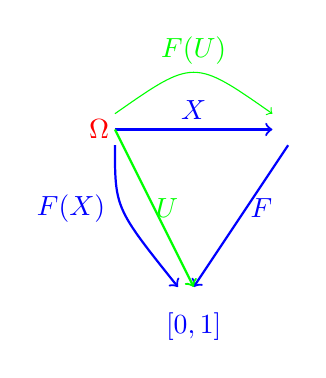
\begin{tikzpicture}
			\draw[blue,thick, ->] (2.2, 2)node{$\bR$}  (0, 2) -- (2,2) ;
			\draw[green] (1.0, 2.7)node[above]{$\geninv{F}(U)$};
			\draw[blue] (1,2.0)node[above]{$X$};
			\draw[blue,thick, ->] (1.0,-0.2)node[below]{$[0,1]$} (2.2,1.8) -- (1.0,0);
			\draw[green, thick, ->] (0,2) -- (1.,0) ;
			\draw[red](-0.2,2)node{$\Omega$};
			\draw[green] (0.4, 1.0)node[right]{$U$};
			\draw[blue] (1.6, 1.0)node[right]{$F$};
			\draw[green,->] (0,2.2) .. controls (1.0, 2.9).. (2.0,2.2);
			\draw[thick, blue, ->] (0, 1.8) .. controls (0,1.0) .. (0.8,0);
			\draw[blue] (0,1.0)node[left]{$F(X)$};
		\end{tikzpicture}
\end{wrapfigure}
	\begin{enumerate}
	\item The following holds true
	\begin{equation}
		\geninv{F}(U) \eqdist X
	\end{equation}
	\item Moreover, if $F$ is continuous then $	F(X) \sim \udist$.
\end{enumerate}